% 1986 年广东卷文史类第 6 题：三棱锥
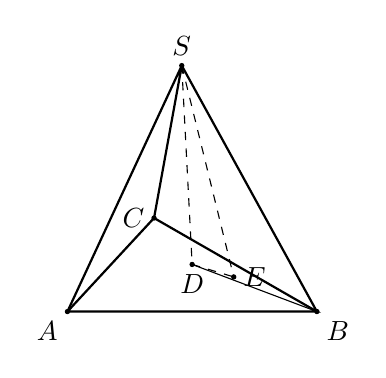
\begin{tikzpicture}[scale=0.88,>=stealth]
  \coordinate (A) at (0,0);
  \coordinate (B) at (3.6,0);
  \coordinate (C) at (1.25,1.35);
  \coordinate (S) at (1.65,3.55);
  \coordinate (D) at (1.8,0.68);
  \coordinate (E) at (2.4,0.5);

  \draw[thick] (A)--(B)--(C)--cycle;
  \draw[thick] (S)--(A) (S)--(B) (S)--(C);
  \draw[dashed] (A)--(C);
  \draw[dashed] (S)--(D) (S)--(E) (D)--(E);
  \draw (D)--(B);
  \fill (A) circle (1.1pt) node[below left] {$A$};
  \fill (B) circle (1.1pt) node[below right] {$B$};
  \fill (C) circle (1.1pt) node[left] {$C$};
  \fill (S) circle (1.1pt) node[above] {$S$};
  \fill (D) circle (1.1pt) node[below] {$D$};
  \fill (E) circle (1.1pt) node[right] {$E$};
\end{tikzpicture}
